%!TEX root=main.tex
\newpage
\subsection{Heurísticas}

\subsubsection{Heurística 1}
%!TEX root=main.tex

A heurística 1, cujo o nome vem do facto de ter sido a primeira a ser implementada, tenta analisar as possibilidades de vitória para ambos os jogadores de uma forma relativamente ingénua. Para explicar como funciona observem-se os seguintes tabuleiros, onde os círculos a verde representam posições ocupadas pelo jogador 1, e a vermelhos as ocupadas pelo jogador 2.

\begin{table}[H]
\centering
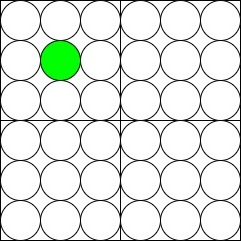
\includegraphics[height=4cm]{images/h1_block1.jpg}
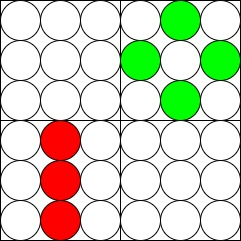
\includegraphics[height=4cm]{images/h1_block2.jpg}
\end{table}

Se atentarmos à segunda linha horizontal, em ambos os tabuleiros, podemos concluir rapidamente que o jogador 2 nunca poderá efetuar quatro em linha na segunda linha horizontal uma vez que esta se encontra bloqueada pelas peças do jogador 1. 

Podemos averiguar que temos 4 conjuntos de posições em cada um dos quadrantes que contêm a segunda linha horizontal. Quando um dos quadrantes fica com os 4 conjuntos ocupados por peças de um jogador deixa de ser possível ao jogador adversário usar essa linha para ganhar o jogo. As figuras seguintes ajudam a ilustrar esta situação no caso da segunda linha horizontal. 

\begin{table}[H]
\centering
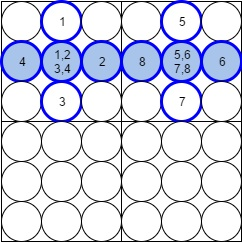
\includegraphics[height=4cm]{images/h1_pattern1.jpg}
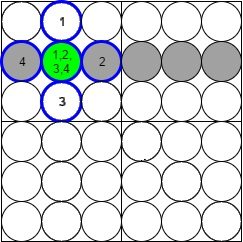
\includegraphics[height=4cm]{images/h1_block3.jpg}
\end{table}

A heurística 1 considera que o \emph{número de possibilidades} que um jogador tem para fazer 5 em linha na segunda linha horizontal é igual ao mínimo número de grupos livres (ainda não ocupados pelo adversário) entre os dois quadrantes que contêm a linha.
Este raciocínio é estendido para as outras linhas que podem ser usadas, sendo no caso das diagonais menores, considerados o mínimo de 3 quadrantes. As figuras seguintes ajudam a perceber o quais os grupos usados para cada linha em cada um dos quadrantes.

\begin{table}[H]
\centering
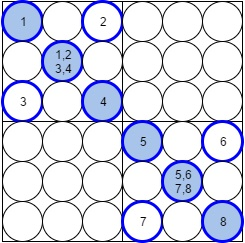
\includegraphics[height=4cm]{images/h1_pattern2.jpg}
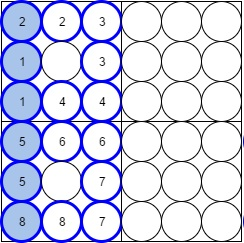
\includegraphics[height=4cm]{images/h1_pattern3.jpg}
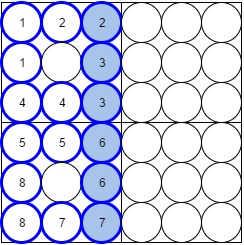
\includegraphics[height=4cm]{images/h1_pattern4.jpg}
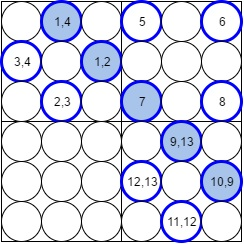
\includegraphics[height=4cm]{images/h1_pattern5.jpg}
\end{table}

A heurística inclui também uma variável \verb|bias| que permite dar mais peso às possibilidades dos jogador ou às possibilidades do jogador adversário. Assim é possível parametrizar a heurística de modo a que tenha um comportamento mais otimista, pessimista, defensivo ou ofensivo. A seguinte fórmula apresenta como é obtido um valor pela heurística, onde $Pm$ é o número de possibilidades para o próprio, $Po$ o número de possibilidades para o oponente e alfa a variável de \verb|bias|.

\begin{equation}
\alpha Pm-(1-\alpha)Po  \qquad\qquad\alpha\in[0,1] 
\end{equation}

Esta consideração é algo ingénua pois é possível que o adversário, fazendo uso das rotações, não permitir o uso de determinadas linhas enganando assim a heurística. Além disso se não é possível usar o minmax para evitar jogadas fatalistas no inicio do jogo, dado existirem demasiadas possibilidades a analisar, a heurística 1, isoladamente, não permite criar um adversário muito forte pois é muito passiva em relação ao estado do tabuleiro, não averiguando derrotas eminentes.

Foram também adicionados pesos aos diversos tipos de linhas. Assim, é possível ao algoritmo priorizar ou desprezar alguns tipos de linhas. Sem entrar em detalhe nos tipos de linhas considerados, intuitivamente estes pesos parecem ser importantes para desprezar as diagonais pequenas que não podem ser usadas em ataques de duas pontas e que ocupam 3 quadrantes. Foi realizada alguma experimentação com estes pesos mas não se chegou a uma solução ideal e não foram realizados testes similares aos apresentados nos anexos dado que já existiam demasiadas variáveis a testar. A adição destas nos testes ia aumentar o número de testes a realizar consideravelmente caso se testasse para todas as possíveis combinações dos \verb|biases|(pesos) na heurística 1 e 1.2.



\subsubsection{Heurística 1.2}
%!TEX root=main.tex

A heurística 1.2 surgiu como na tentava de melhorar a heurística 1. Esta heurística faz o que a sua predecessora já fazia e adicionalmente mais algumas avaliações semelhantes que visão evitar jogadas fatalistas ou aproveitar oportunidades ofensivas. Para tal a heurística considera além do \emph{número de possibilidades} o \emph{número de possibilidades fortes}. 
Para explicar o que o algoritmo entende como possibilidades fortes vamos atentar a segunda linha horizontal do tabuleiro do Pentago. 

\begin{table}[H]
\centering
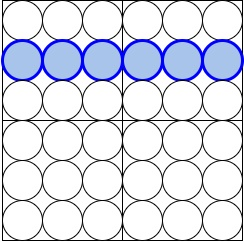
\includegraphics[height=3.5cm]{images/h12_hline.jpg}
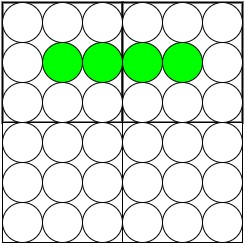
\includegraphics[height=3.5cm]{images/h12_fatal.jpg}
\end{table}

Podemos observar que o tipo de padrão usado na figura à direita é interessante do ponto de vista ofensivo, pois cria uma vitória garantida, e é contra este género de situações que o algoritmo tenta precaver-se ou tirar proveito ofensivo.
Para tal, o algoritmo contabiliza 2 tipos de casos. Denominemos esses tipos de tipo \emph{forte} e de tipo \emph{muito forte} sendo que qualquer caso que seja do tipo muito forte é também um caso do tipo forte mas o inverso pode não ser verdade. Considera-se um caso forte quando um grupo, dos definidos na heurística 1, está ocupado por peças de um jogador. Um caso muito forte acontece quando um grupo está ocupado por peças de um jogador e a sua extensão no mesmo quadrante se encontra sem uma peça adversária (podendo estar vazia ou não). Assim as 3 imagens seguintes ilustram respetivamente 2 jogadas do tipo muito forte e uma do tipo forte.

\begin{table}[H]
\centering
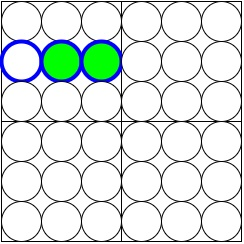
\includegraphics[height=3.5cm]{images/h12_VS.jpg}
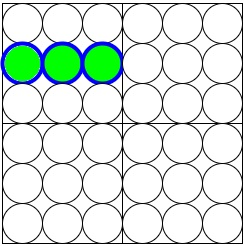
\includegraphics[height=3.5cm]{images/h12_VS2.jpg}
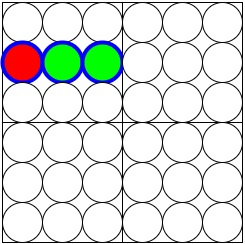
\includegraphics[height=3.5cm]{images/h12_S.jpg}
\end{table}

Depois de contabilizadas estes casos o número de jogadas fortes para a segunda linha horizontal é dada pela seguinte fórmula:
\begin{equation}
F_hor2 = max( min(F_1,M_1) , min(M_2,F_2) )
\end{equation}
Onde $Fi$ e $Mi$ representam respetivamente o número de casos fortes e o número de casos muito fortes no quadrante $i$. Os quadrantes usados, são os que contêm a linha como mostra a figura seguinte.

\begin{table}[H]
\centering
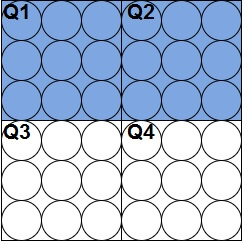
\includegraphics[height=3.5cm]{images/boardsQuadrants.jpg}
\end{table}

Assim, para melhor ilustrar a contabilização referida, são apresentadas abaixo exemplos onde o número de jogadas fortes para a segunda linha horizontal são respetivamente 1, 1, 1 e 2.

\begin{table}[H]
\centering
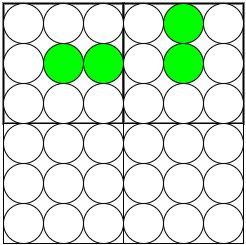
\includegraphics[height=4cm]{images/h12_ex1.jpg}
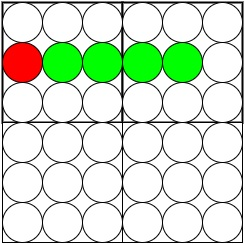
\includegraphics[height=4cm]{images/h12_ex2.jpg}
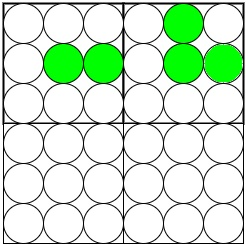
\includegraphics[height=4cm]{images/h12_ex3.jpg}
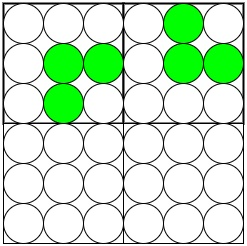
\includegraphics[height=4cm]{images/h12_ex4.jpg}
\end{table}

A mesmos cálculos são efetuados para as outras linhas (excluindo s diagonais menores que são tratadas de forma diferente) para ambos os jogadores. A heurística usa o número de jogadas fortes para o jogador (com valor positivo), para adversário (com valor negativo) e também as possibilidades da heurísticas 1. Todas estas componentes têm um peso associado que confere à heurística alguma flexibilidade podendo esta variar não só entre uma abordagem otimista ou pessimista mas também por abordagem mais passiva ou reativa.

Apesar destas considerações a heurística têm algumas dificuldades em lidar com  limitações de profundidade no Minmax pelo que foi implantada uma versão relaxada. Na sua versão relaxada consideram-se como fortes os blocos ocupados com pelo menos uma peça do jogador e nenhuma do adversário, tal como apresentado na ilustração abaixo.

\begin{table}[H]
\centering
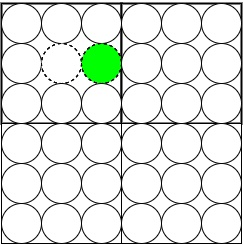
\includegraphics[height=4cm]{images/h12_relax.jpg}
\end{table}

Apesar de melhorar a sua predecessora também herda as suas fraquezas não sabendo lidar com as rotações do jogador adversário.



\subsubsection{Heurística A}
%!TEX root=main.tex

Esta heurística foi inspirada pelo guia estratégico~[2].

Há 4 formas de obter 5 em linha e ganhar um jogo de Pentago:
\begin{itemize}
	\item Monica - numa das diagonais principais do tabuleiro - força relativa 3
\begin{table}[H]
\centering
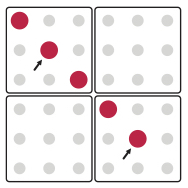
\includegraphics[height=3.7cm]{images/monica.jpg}
\end{table}
	\item Meio - na vertical ou na horizontal através do meio de dois quadrantes adjacentes - força relativa 5
\begin{table}[H]
\centering
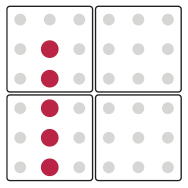
\includegraphics[height=3.7cm]{images/middle.jpg}
\end{table}
	\item Direito - na vertical ou na horizontal usando os bordos de dois quadrantes adjacentes - força relativa 7
\begin{table}[H]
\centering
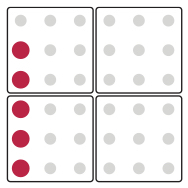
\includegraphics[height=3.7cm]{images/straight.jpg}
\end{table}
	\item Tripla - diagonalmente, abaixo ou acima das diagonais principais do tabuleiro - força relativa 9
\begin{table}[H]
\centering
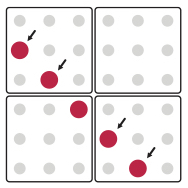
\includegraphics[height=3.7cm]{images/triple.jpg}
\end{table}
\end{itemize}

Para cada uma destas estratégias, considera-se a sua versatilidade, isto é, o número de diferentes possibilidades de aproveitar parte das peças quando um dos caminhos é bloqueado pelo adversário. Além disso, também nos interessa a dificuldade que o adversário tem de se defender contra um jogador que use a estratégia. São esses dois fatores que determinam a força relativa.

Dada uma posição do jogo, a heurística A começa por percorrer cada uma das linhas em que é possível ganhar e calcular o número de peças de cada cor. No entanto, apenas nos interessa contabilizar as peças quando há possibilidade do jogador conseguir ganhar nessa linha. Para isso, vamos verificar quantas peças há no interior da linha e quantas peças há nos bordos, dado que peças do adversário no interior bloqueiam imediatamente e para bloquear nos bordos são necessárias duas peças. Depois de efetuada esta contagem, sabemos quão forte é a posição de cada jogador em cada linha. Por exemplo, se há 3 peças brancas no interior e nenhuma peça preta em toda a linha, a posição branca é muito forte, porque basta mais uma peça para assegurar a sua vitória. 

No passo seguinte, usamos as forças relativas e as contagens para calcular o valor do tabuleiro. Sendo~$b$ o número de peças brancas,~$p$ o número de peças pretas e~$r$ a força relativa na linha em questão, adicionamos~$r^b - r^p$ ao valor previamente calculado. Este valor está a ser calculado assumindo que a IA está a jogar com as peças brancas, mas caso esteja a jogar com as pretas, basta multiplicar por -1 no final. O motivo pelo qual usamos a potência, é para garantir que ter várias peças na mesma linha é mais valorizado do que ter as mesmas peças espalhadas por linhas diferentes.

O método acima é usado para calcular o valor de todos os 8 tabuleiros que se obtém do tabuleiro atual por rotação de um quadrante. Depois disso, é usado o máximo ou o mínimo destes tabuleiros rodados, consoante o próximo jogador é a IA ou o adversário, tal como no minmax.

Em relação às forças relativas, apesar de querermos favorecer determinadas estratégias em detrimento de outras, não usamos os valores 3, 5, 7, e 9, porque devido ao uso de potências, eles conduzem a discrepâncias enormes entre jogadas, que fariam com que algumas das estratégias fossem completamente desprezadas. Sendo assim, após alguns cálculos com várias posições de jogo, optamos pelos valores 1.13, 1.15, 1.17 e 1.19. Isto contribui também para que os valores finais do tabuleiro sejam pequenos, o que será usado noutras considerações da heurística como veremos adiante. Dada a arbitrariedade da escolha dos valores, decidimos efetuar experiências estatísticas para determinar os melhores valores, mas isso será visto mais adiante na secção das experiências.

Observando jogos em que a heurística A perdia, rapidamente conseguimos determinar algumas das suas falhas. A primeira destas observações é que se um jogador conseguir 4 em linha com as duas pontas abertas (em jogadas do tipo monica, meio ou direito), então irá ganhar na próxima jogada, a não ser que o seu adversário ganhe já nesta. Assim, ao detetar estas situações a heurística A ignora todos os outros cálculos e dá valor 100 ao tabuleiro se ganha e -100 se perde.

Outra maneira certa de ganhar é conseguir duas ou mais linhas em que apenas falta uma peça para ganhar. Estas situações também foram introduzidas como exceção na heurística A, embora possam levar a alguns falsos positivos, quando ambas as linhas de vitória necessitam de uma peça na mesma posição do tabuleiro.

Finalmente, fizemos ainda algumas pequenas alterações aos valores da heurística:
\begin{itemize}
	\item se tivermos 4 peças em linha com as pontas abertas, mas for a vez do adversário, calculamos o valor como se fossem 10 peças, para que seja claramente mais valorizada que as restantes;
	\item se faltar apenas uma peça para obter 5 em linha e não estivermos na situação anterior, incrementamos a contagem de peças em 1;
	\item se houver 1, 2 ou 3 peças não bloqueadas na mesma linha (monica, meio ou direito), como ambas as pontas abertas, incrementamos a contagem em 1.
\end{itemize}

\subsubsection{Heurística A hacked}

A heurística A hacked não apresenta nenhuma construção nova face às anteriores. Na verdade apenas aparece na secção de especificação para ser referida na mesma secção das outras heurísticas neste relatório. A heurística A hacked resulta de experimentação, tendo sido descoberto, combinando pesos das diferentes heurísticas implementadas, que a heurística A tinha alguma facilidade em perder nas diagonais principais. A heurística A hacked apareceu como uma contra-heurística à A fazendo uso de funcionalidades da heurística 1.2 para evitar perder nas diagonais principais. Atualmente a heurística A star apresenta melhores resultados ao usar uma profundidade de 4 (2 jogadas).

\subsubsection{Heurística A star}

Esta heurística é uma melhoria da heurística A. A ideia básica é a mesma, mas introduzimos mais algumas verificações e alteramos outras. Além disso, nesta heurística também é possível determinar se se estudam todos os tabuleiros rodados quando a jogada é de rotação. No entanto, como veremos na secção das experiências, o desempenho da heurística é melhor quando se estudam todas as rotações.

Uma das mudanças essenciais nesta heurística é que há uma maior preocupação com quem é o próximo jogador a jogar. Por exemplo, imaginemos que ambos os jogadores têm 4 em linha com as duas pontas abertas. Então, quem irá ganhar é o próximo a jogar. Por outro lado, se apenas um dos jogadores estiver nessa posição, mesmo que não seja a vez dele, ele irá ganhar a seguir, a não ser que o outro ganhe antes por outra situação. Sendo assim, há que estudar em todos os tabuleiros rodados, quais as possibilidades de vitória dos dois jogadores. O próximo a jogar apenas precisa que um dos rodados lhe dê vitória. Enquanto que o outro precisa que um dos rodados lhe dê vitória e nenhum dê ao seu adversário.

Outra mudança significativa tem a ver com possibilidades de vitória, ainda que não seja certa. Isto é, com situações em que um dos jogadores ganha, a não ser que o outro o impeça. Nesses casos o tabuleiro é classificado com os valores 50 ou -50 consoante é o jogador computador que tem a possibilidade de ganhar ou o seu adversário. Mais uma vez, isto é estudado tendo em conta todos os rodados e quem é o próximo a jogar.

Em vários aspetos, esta heurística efetua correções à heurística A, isto é, calcula o valor da forma que realmente se pretendia fazer em A, mas que pela complexidade da heurística não foi inicialmente conseguido. No entanto, como a performance da A por vezes é melhor que a da A star, optamos por manter as duas heurísticas no jogo.

Usando profundidade 4, a profundidade máxima que se pode usar nas nossas máquinas que ainda obtém uma reposta imediata do ponto de vista do utilizador, esta é a única heurística que com os valores das forças relativas default consegue precaver-se contra uma tática ofensiva específica no Pentago. Ao controlar o centro dos quadrantes e atacar pelas diagonais as outras heurísticas perdem se não usarem profundidades mais elevadas. 